

\section{Bowtie2}

\subsection{Experiment}

I wrote a simple python script that would grab a list of all the virus genomes at a given location (either Victoria, Toronto, or Carlon in this case), then download the genome and align it against the reference index using Bowtie2. Each node had to have a local copy of the reference index and so I got the script to grab it from the Bowtie2 sourceforge site. I could have stored the reference in the distributed filesystem, but the reference index is $3.5$ GB and there was not enough space in the filesystem to store it. Normally $3.5$ GB would not be a problem but the filesystem is a prototype and I wanted it to have a minimal footprint on the machines where it runs. 

After the reference had been downloaded the node could start processing. For a given virus genome the node would grab it out of the sage filesystem and transfer it to the local filesystem (a function provided with sage), as the sage client is simply a python interface to the remote location and Bowtie2 is a standalone binary. Then Bowtie2 was run with default local scoring parameters looking for a local alignment comparing the virus sequence to the human sequence. As a sight aside, the memory on the nodes had to be increased from $512$ MB to at least $4$ GB to run Bowtie2. The memory was actually increased to $8$ GB on all the nodes as MUMmer required more than $4$ GB. After the alignment was finished the output file was placed back into sage. It took upwards of $36$ hours to to align all $5534$ sequences and produce the results. Bowtie2 reports if a suitable match was found, and has more information on the match about where it occurs and what the alignment looks like. The results found by Bowtie2 are summarized in Table \ref{tab:bowtieresults} and presented in Figure \ref{fig:bowtieplot}.



\begin{table*}
\caption{Matching Sequence Found Using Bowtie2.}
\begin{center}
\begin{tabular}{llllll}
\hline\noalign{\smallskip}
NCBI Name & Ref. & Chrom. & Max Match & Tot Match & Tot Seq \\
\hline\noalign{\smallskip}

Abelson\_murine\_leukemia\_virus\_uid14654 & NC\_001499 & chr9 & $207$ & $232$ & $5894$ \\
Alternaria\_alternata\_dsRNA\_mycovirus\_uid30367 & NC\_010989 & chr21 & $41$ & $41$ & $2794$ \\
Alternaria\_alternata\_dsRNA\_mycovirus\_uid30367 & NC\_010991 & chr5 & $37$ & $37$ & $1420$ \\
Aspergillus\_foetidus\_dsRNA\_mycovirus\_uid186431 & NC\_020101 & chr1 & $41$ & $41$ & $2466$ \\
Aspergillus\_foetidus\_dsRNA\_mycovirus\_uid186431 & NC\_020102 & chr5 & $41$ & $41$ & $2005$ \\
Avian\_myelocytomatosis\_virus\_uid14909 & NC\_001866 & chr8 & $151$ & $203$ & $3392$ \\
Broad\_bean\_mottle\_virus\_uid14833 & NC\_004006 & chr3 & $40$ & $40$ & $2293$ \\
Cassia\_yellow\_blotch\_virus\_uid15419 & NC\_007001 & chrX & $42$ & $42$ & $2091$ \\
Cotesia\_congregata\_bracovirus\_uid14556 & NC\_006641 & chr2 & $59$ & $60$ & $15960$ \\
Cotesia\_congregata\_bracovirus\_uid14556 & NC\_006647 & chr3 & $52$ & $52$ & $8785$ \\
Cowpea\_chlorotic\_mottle\_virus\_uid14758 & NC\_003542 & chr5 & $39$ & $39$ & $2173$ \\
Dill\_cryptic\_virus\_1\_uid225921 & NC\_022614 & chr9 & $39$ & $39$ & $2013$ \\
Dill\_cryptic\_virus\_1\_uid225921 & NC\_022615 & chrX & $33$ & $44$ & $1837$ \\
Dill\_cryptic\_virus\_2\_uid198774 & NC\_021148 & chr6 & $44$ & $44$ & $2354$ \\
Glypta\_fumiferanae\_ichnovirus\_uid18767 & NC\_008862 & chrX & $51$ & $52$ & $2299$ \\
Glypta\_fumiferanae\_ichnovirus\_uid18767 & NC\_008895 & chr5 & $45$ & $45$ & $2854$ \\
Glypta\_fumiferanae\_ichnovirus\_uid18767 & NC\_008908 & chr22 & $53$ & $55$ & $3084$ \\
Glypta\_fumiferanae\_ichnovirus\_uid18767 & NC\_008912 & chr2 & $181$ & $423$ & $3179$ \\
Glypta\_fumiferanae\_ichnovirus\_uid18767 & NC\_008913 & chr3 & $86$ & $134$ & $3157$ \\
Glypta\_fumiferanae\_ichnovirus\_uid18767 & NC\_008925 & chr12 & $82$ & $90$ & $3821$ \\
Groundnut\_ringspot\_and\_Tomato\_chlorotic\_spot\_virus\_reassortant\_uid66459 & NC\_015467 & chr12 & $41$ & $41$ & $3067$ \\
HCBI8\_215\_virus\_uid257701 & NC\_024689 & chr5 & $69$ & $69$ & $2152$ \\
Hepatitis\_C\_virus\_genotype\_6\_uid20939 & NC\_009827 & chr17 & $58$ & $58$ & $9628$ \\
Hepatitis\_C\_virus\_uid15432 & NC\_004102 & chr14 & $47$ & $47$ & $9646$ \\
Hibiscus\_latent\_Singapore\_virus\_uid17573 & NC\_008310 & chr5 & $49$ & $49$ & $6474$ \\
Human\_endogenous\_retrovirus\_K113\_uid222261 & NC\_022518 & chr4 & $1222$ & $2552$ & $9716$ \\
Hyposoter\_fugitivus\_ichnovirus\_uid18779 & NC\_008962 & chr12 & $55$ & $55$ & $3385$ \\
Hyposoter\_fugitivus\_ichnovirus\_uid18779 & NC\_008969 & chr14 & $46$ & $51$ & $3958$ \\
Jingmen\_Tick\_Virus\_uid247973 & NC\_024112 & chr6 & $43$ & $53$ & $2850$ \\
Mason\_Pfizer\_monkey\_virus\_uid14683 & NC\_001550 & chr15 & $59$ & $59$ & $8557$ \\
Murine\_osteosarcoma\_virus\_uid14655 & NC\_001506 & chr11 & $134$ & $135$ & $3811$ \\
Oyster\_mushroom\_spherical\_virus\_uid14951 & NC\_004560 & chr7 & $41$ & $69$ & $5799$ \\
Pestivirus\_Giraffe\_1\_uid14780 & NC\_003678 & chr12 & $163$ & $202$ & $12646$ \\
Phytophthora\_infestans\_RNA\_virus\_1\_uid40329 & NC\_013221 & chr4 & $41$ & $41$ & $2896$ \\
Pleurotus\_ostreatus\_virus\_uid15169 & NC\_006960 & chr3 & $47$ & $47$ & $2223$ \\
Raspberry\_latent\_virus\_uid56055 & NC\_014602 & chr10 & $43$ & $46$ & $2565$ \\
\hline\noalign{\smallskip}
\end{tabular} 
\end{center}
\label{tab:bowtieresults}
\end{table*}



\begin{figure*}
\caption{Plot of Matching Sequence vs Total Sequence}
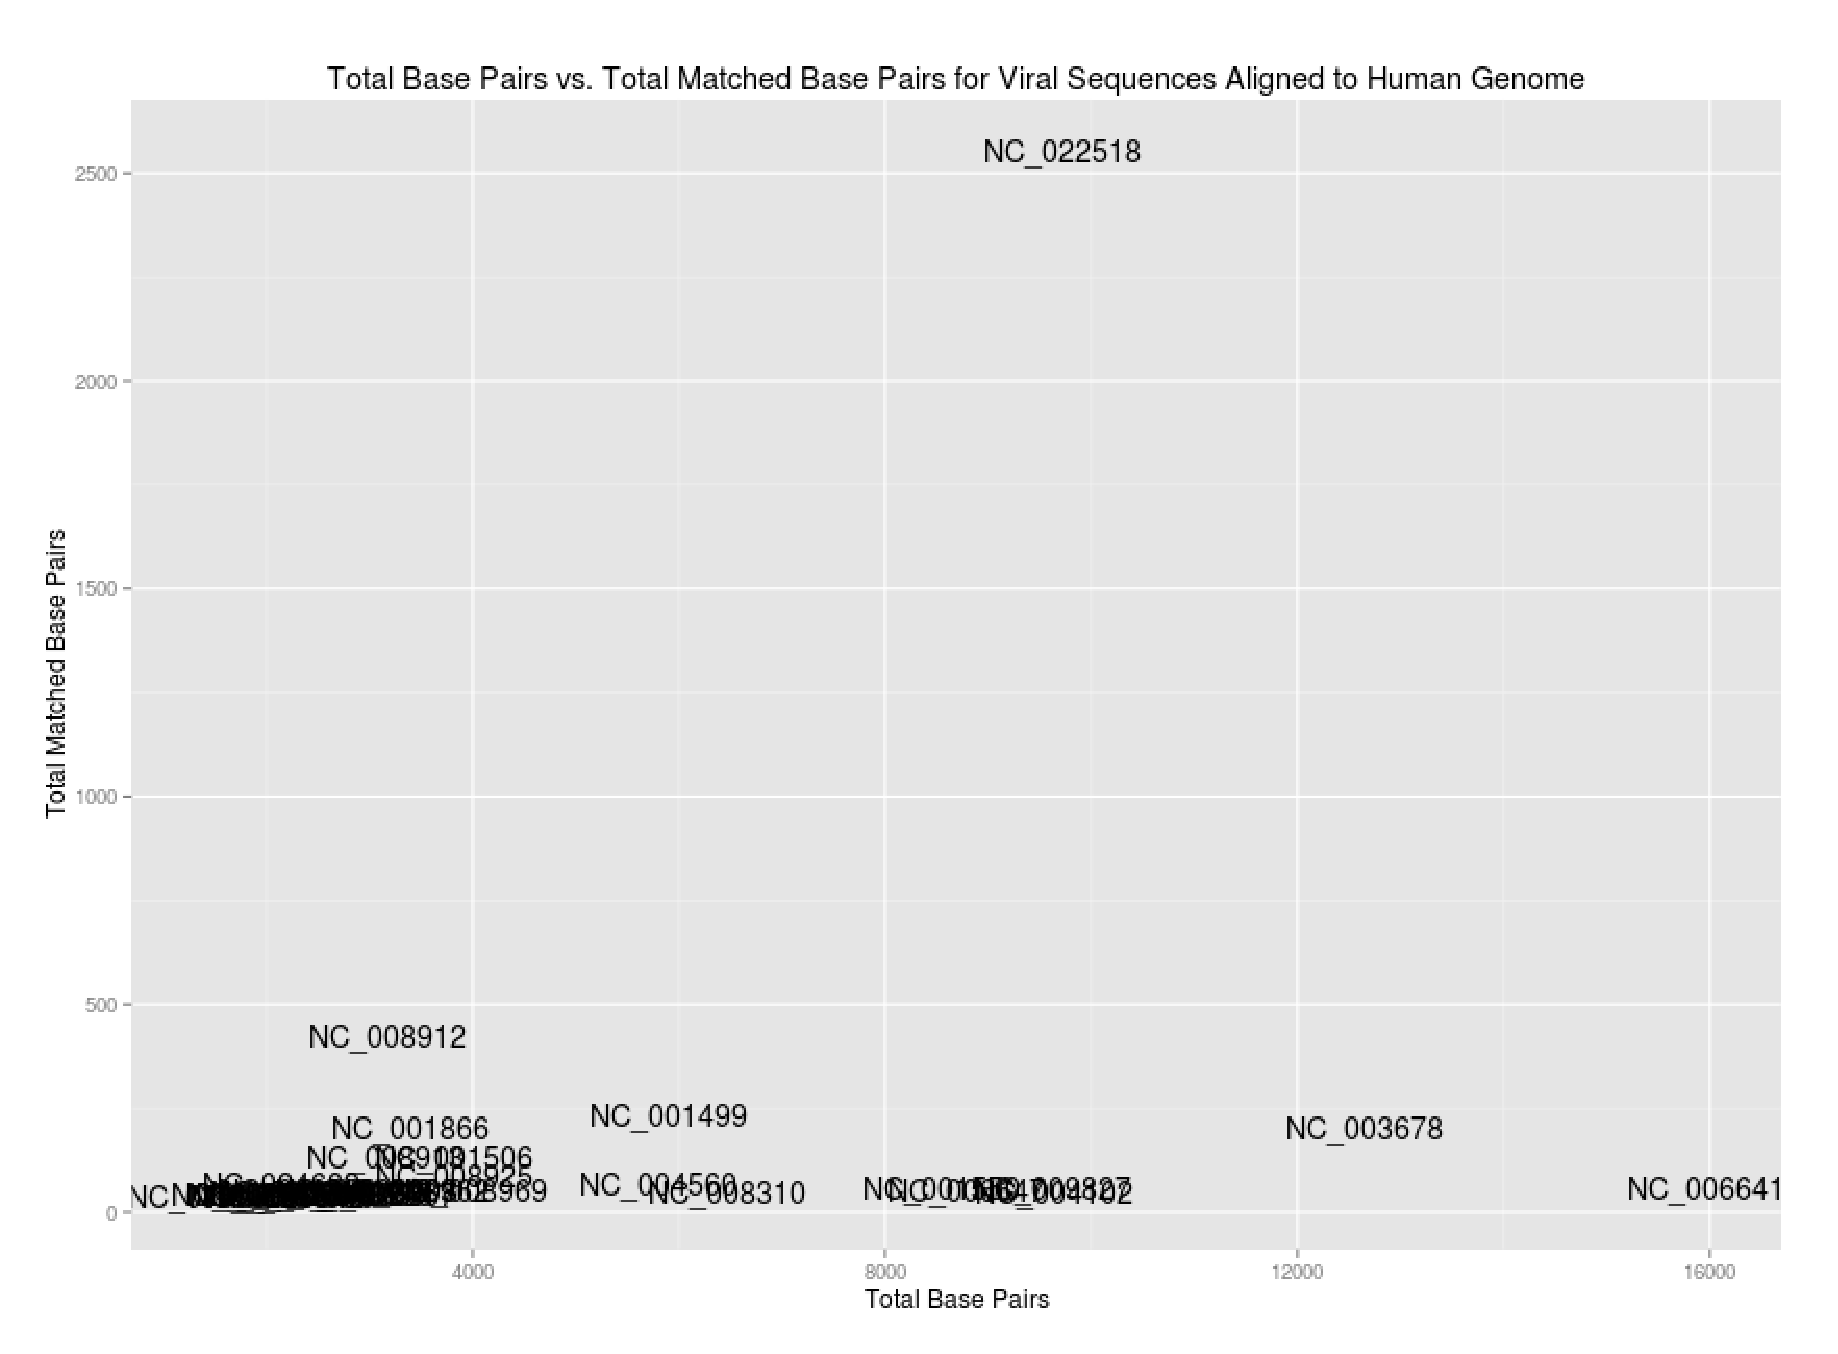
\includegraphics[width=\textwidth]{img/bowtie2results.eps}
\label{fig:bowtieplot}
\end{figure*}




\subsection{Results}

Of the $5534$ alignments performed only $36$ probable alignments were found. Of the $36$ none were particularly long alignments, the largest being HERV-K113 with approximately a quarter of the viral sequence aligned to chromosome $4$. This is somewhat surprising as HERV-K113 is only found within the human genome. Most of the alignments are likely false positives not actually representing gene transfer as for such small sequences It is far more likely to be random chance. This may seem like somewhat of a negative result, but it really shows that EVEs are more elusive than I previously thought. This is not amazingly surprising as many of these fragments have existed in our genome for millions of years, so it is not hard to imagine the sequences have diverged over time. Additionally the places where these fragments are inserted are somewhat volatile. In fact if such elements are inserted into critical genes, a disease state would likely occur. From the results obtained and the knowledge that the sequences are most likely not conserved I decided to look at a more sensitive alignment using MUMmer.